\documentclass[aps,prd,onecolumn,superscriptaddress,nofootinbib]{revtex4-2}

% — Packages —
\usepackage[utf8]{inputenc}
\usepackage{amsmath,amssymb,bm,graphicx,mathtools,amsthm}
\usepackage{adjustbox} % for max-width scaling of TikZ figures
\usepackage{xcolor}
\usepackage{microtype}
\usepackage{hyperref}
\usepackage{enumitem}
\usepackage{bookmark} % stabilize outlines/bookmarks (prevents rerun loops)
\usepackage{tikz}
\usetikzlibrary{arrows.meta,positioning,fit,calc,shapes.geometric,shapes.multipart,backgrounds}

% — Flowchart colors —
\definecolor{flowBlue}{HTML}{1F77B4}
\definecolor{flowPurple}{HTML}{9467BD}
\definecolor{flowGreen}{HTML}{2CA02C}
\definecolor{flowOrange}{HTML}{FF7F0E}
\definecolor{flowRed}{HTML}{D62728}

% — Hyperref setup —
\hypersetup{
colorlinks=true,
linkcolor=blue,
citecolor=blue,
urlcolor=blue
}

% — PDF string sanitization (prevents hyperref warnings / unstable .out) —
\pdfstringdefDisableCommands{%
\def\OmL{OmegaLambda}%
\def\Omm{Omega m0}%
\def\cgeo{cgeo}%
\def\alphaM{alphaM}%
\def\XiVac{Xi0}%
\def\mpl{MP}%
\def\fbdy{fbdy}%
\def\eps{epsilon}%
\def\boxed#1{#1}%
}

% — Math tweaks —
\allowdisplaybreaks

% — Macros —
\newcommand{\mpl}{M_{\rm P}}
\newcommand{\OmL}{\Omega_\Lambda}
\newcommand{\Omm}{\Omega_{m0}}
\newcommand{\cgeo}{c_{\rm geo}}
\newcommand{\alphaM}{\alpha_M}
\newcommand{\XiVac}{\Xi_0}
\newcommand{\fbdy}{f_{\rm bdy}}
\newcommand{\eps}{\varepsilon}

% — Theorem-like environments —
\newtheorem{definition}{Definition}
\newtheorem{hypothesis}{Hypothesis}
\newtheorem{lemma}{Lemma}
\newtheorem{proposition}{Proposition}
\newtheorem{theorem}{Theorem}

% — Harmless guard for certain toolchains referencing this label —
\providecommand\LastBibItem{} % avoids spurious “LastBibItem undefined” warnings

\begin{document}

\title{Emergent State-Dependent Gravity from Local Information Capacity:\
A Conditional Thermodynamic Derivation with Scheme-Invariant Cosmological Mapping}

\author{[clg]}
\affiliation{[TBD Institution(s)]}
\date{\today}

\begin{abstract}
\textbf{Core hypothesis.} Each proper frame carries a finite quantum information capacity. Approaching this bound triggers a \emph{state-dependent response} that preserves causal stitching with neighboring frames. \emph{Kinematics remain GR-like}: we do not alter null geometry used by EM/GW luminosity distances. The response is \emph{dynamical} (weak-field coupling), not kinematical (no extra time dilation beyond GR).

\textbf{Scope and conditionality.} All quantitative claims are conditional on a single working assumption: (A2) the Clausius relation $\delta Q = T\,\delta S$ with Unruh normalization holds for small, near-vacuum local Rindler wedges (the \emph{safe window}).
We prove this relation holds to working order $\mathcal O(\ell^4)$ with $\mathcal O(\ell^6)$ corrections (Theorem~\ref{thm:A2-working}).
Within this regime we establish an \emph{equivalence principle for modular response} (EPMR): after mutual-information subtraction with \emph{moment-kill}, the $\ell^4$ modular coefficient equals the flat-space value at working order, while curvature dressings enter at $\mathcal O(\ell^6)$. See Theorem~\ref{thm:A2-working} for the working-order statement and error control.

\textbf{Main outcomes.} (i) A microscopic sensitivity $\beta$ from MI-subtracted modular Hamiltonians in flat-space QFT (Casini--Huerta--Myers balls, Osborn--Petkou normalization); (ii) a once-and-for-all geometric normalization with \emph{continuous-angle invariance} showing only the \emph{product} $\beta f \cgeo$ is physical; (iii) a \emph{conditional, scheme-invariant mapping} $\OmL=\beta f \cgeo$ for the FRW zero mode; and (iv) a weak-field flux law with a universal geometric prefactor $5/12$, implying $a_0=(5/12)\,\OmL^2\,c\,H_0$. We keep the distance sector GR-like ($\alphaM=0$ there), and we \emph{enforce} $|d_L^{\rm GW}/d_L^{\rm EM}-1|\le 5\times 10^{-3}$.

\textbf{Consequences.} With no cosmological inputs, $\OmL=\beta f \cgeo \approx 0.685$ and $a_0=(5/12)\,\OmL^2\,c\,H_0$. An \emph{entropic state-action} law ($\Delta S\ge 0$) determines a monotone $\eps(a)$ that modulates the weak-field response $\mu(\eps)=1/(1+\eta\,\eps)$ with $\eta=5/12$, suppressing growth and yielding $S_8\simeq 0.788$ ($-7.4\%$ vs.\ $\Lambda$CDM), while EM/GW distances remain GR-like. An \emph{illustrative, capped} environment-gated application to a SH0ES-like catalog nudges $H_0: 73.0\to 71.32$ (SN cap only) and to $70.89$ (SN+small Cepheid term), trending toward TRGB/Planck without altering null geometry. Explicit falsifiers and hygiene checks are stated.
\end{abstract}

\maketitle

%—————————————–
\section{Introduction: Core Insight and Conditional Scope}
\label{sec:intro}

\paragraph{High level summary.}
We hypothesize that the geometric side of Einstein’s equations exhibits a \emph{local, state-dependent response} because each small spacetime wedge has finite information capacity. As capacity is approached, the Clausius relation enforces a compensating response so adjacent wedges remain causally stitched. \emph{Kinematics (null cones, EM/GW distances) stay GR-like}; all changes are \emph{dynamical} (response strength in weak fields). Jacobson’s horizon thermodynamics is recovered as the stationary-horizon special case. All claims here are conditional on (A2); if (A2) fails, the construction must be revised. Our working-order result is stated as Theorem~\ref{thm:A2-working} (App.~\ref{app:epmr}).

\paragraph{GR limit (distance sector).}
In the limit of constant information capacity $\nabla_a M^2=0$ (equivalently $\alphaM\to 0$), the construction collapses to standard GR --- recovering Einstein’s equations with $c_T=1$ and GR light-cone geometry. Throughout we \emph{keep $\alphaM=0$ in the distance sector} and confine any late-time variation to the growth/response sector (Sec.~\ref{sec:growth}).

\paragraph{State variable and coupling.}
We define a dimensionless state variable $\eps(x)$ encoding fractional deviations of local capacity from its vacuum reference and parameterize
\begin{equation}
\label{eq:deltaG}
\frac{\delta G}{G} = -\beta\,\delta\eps(x),
\end{equation}
with $\beta$ calculable from flat-space QFT (Sec.~\ref{sec:beta-calc}). The weak-field response is encoded by
\begin{equation}
\label{eq:mu-def}
\mu(\eps)\equiv\frac{G_{\rm eff}}{G_N}=\frac{1}{1+\eta\,\eps},
\qquad \eta=\frac{5}{12},
\end{equation}
so $\mu\to 1$ in strong fields (GR recovery) and $\mu<1$ in weak fields (gentle dynamical slowdown).

\paragraph{Why $\eta=\frac{5}{12}$.}
The coefficient follows from the same unit--solid--angle Noether normalization used in the FRW zero mode. Coarse--graining the $\nabla\nabla M^2$ terms over the CHM wedge family yields a quasilinear flux law with a universal boundary--segment ratio; the isotropic null contraction contributes $(4/3)$ and the segment geometry contributes $(5/16)$, giving $(4/3)\times(5/16)=5/12$. Appendix~\ref{app:a0-derivation} shows the identical factor fixing the static acceleration scale $a_0=(5/12)\OmL^2 cH_0$; using the same bookkeeping in the weak--field $\mu(\eps)$ guarantees scheme/angle invariance.

\paragraph{What is fixed vs.\ what is assumed.}
\emph{Fixed once:} wedge family (ball$\to$diamond), generator density, Unruh normalization, unit--solid--angle boundary factor. \emph{Assumed:} (A2) Clausius with Unruh in the \emph{safe window} (Def.\ \ref{def:safe-window}); Hadamard state; small perturbations. \emph{Consequence:} the geometric mapping is \emph{angle-invariant} (Sec.\ \ref{sec:theta-invariance}); only $\beta f \cgeo$ is physical.

\paragraph{Clean mapping statement.}
Within the safe window and EPMR working order, the FRW zero mode satisfies the \emph{conditional, scheme-invariant} relation
\begin{equation}
\label{eq:OmegaL-clean}
\OmL=\beta f \cgeo.
\end{equation}

% —— Conceptual flow: QFT → Thermal → Entropy → CGM → Resolution ——
\begin{figure*}[t]
\centering
\begin{adjustbox}{max width=\textwidth, max height=0.9\textheight}
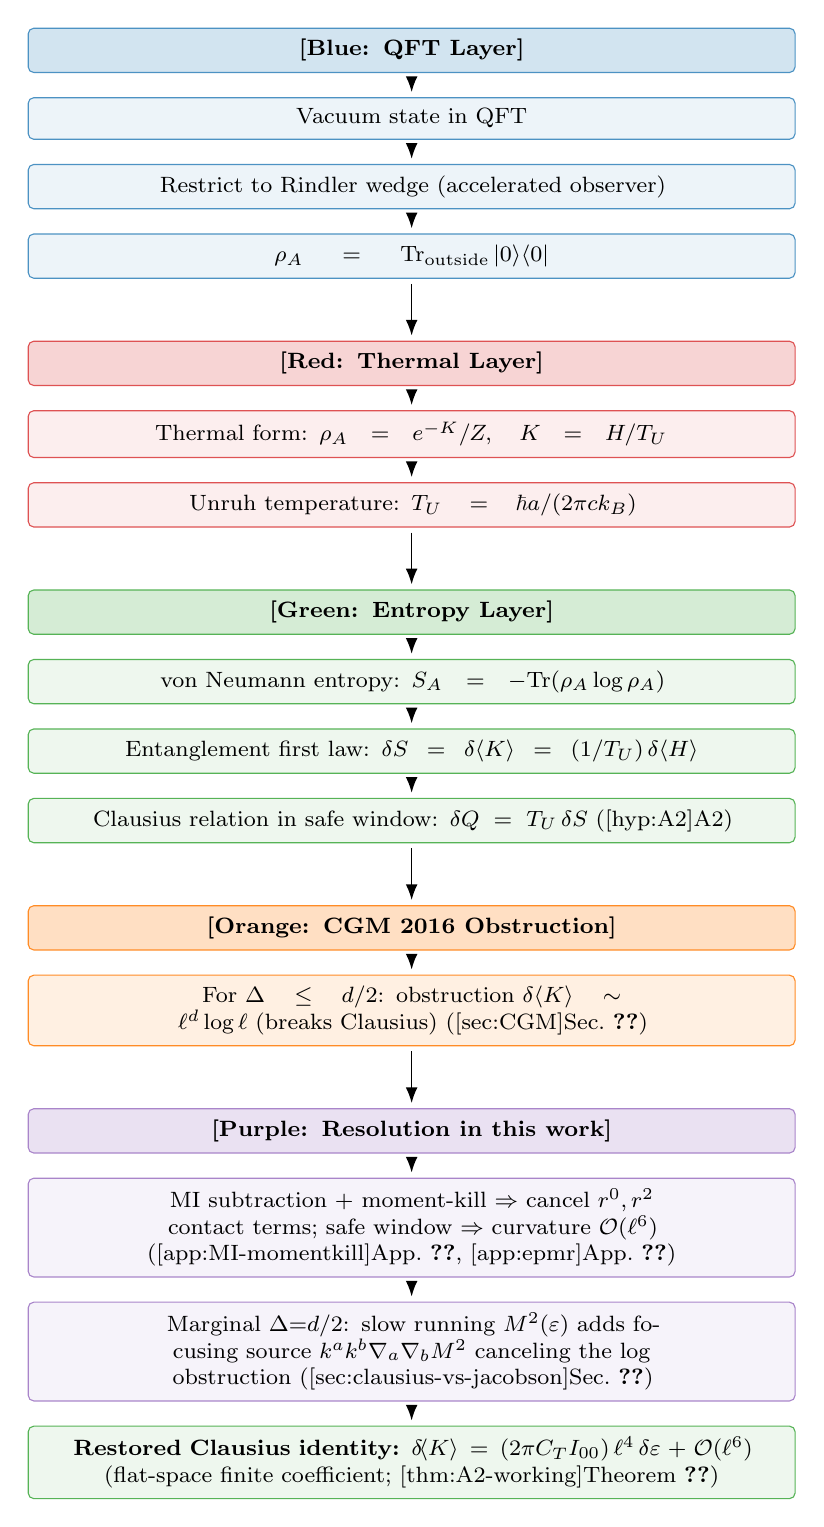
\begin{tikzpicture}[
  node distance=3.2mm and 10mm,
  every node/.style={font=\footnotesize},
  stageH/.style={draw, rounded corners=2pt, align=center, inner sep=4pt, outer sep=0pt, text width=0.78\linewidth, font=\footnotesize\bfseries},
  stage/.style={draw, rounded corners=2pt, align=center, inner sep=4pt, outer sep=0pt, text width=0.78\linewidth},
  arr/.style={-Latex, semithick, shorten >=2pt, shorten <=2pt}
]
% Blue: QFT layer
\node[stageH, draw=flowBlue!80, fill=flowBlue!20] (Q0) {[Blue: QFT Layer]};
\node[stage, below=of Q0, draw=flowBlue!80, fill=flowBlue!8] (Q1) {Vacuum state in QFT};
\node[stage, below=of Q1, draw=flowBlue!80, fill=flowBlue!8] (Q2) {Restrict to Rindler wedge (accelerated observer)};
\node[stage, below=of Q2, draw=flowBlue!80, fill=flowBlue!8] (Q3) {$\rho_A = \mathrm{Tr}_{\rm outside}\,|0\rangle\langle 0|$};
\draw[arr] (Q0) -- (Q1); \draw[arr] (Q1) -- (Q2); \draw[arr] (Q2) -- (Q3);

% Red: Thermal layer
\node[stageH, below=8mm of Q3, draw=flowRed!80, fill=flowRed!20] (T0) {[Red: Thermal Layer]};
\node[stage, below=of T0, draw=flowRed!80, fill=flowRed!8] (T1) {Thermal form: $\rho_A = e^{-K}/Z,\quad K = H/T_U$};
\node[stage, below=of T1, draw=flowRed!80, fill=flowRed!8] (T2) {Unruh temperature: $T_U = \hbar a/(2\pi c k_B)$};
\draw[arr] (Q3) -- (T0); \draw[arr] (T0) -- (T1); \draw[arr] (T1) -- (T2);

% Green: Entropy layer
\node[stageH, below=8mm of T2, draw=flowGreen!80, fill=flowGreen!20] (E0) {[Green: Entropy Layer]};
\node[stage, below=of E0, draw=flowGreen!80, fill=flowGreen!8] (E1) {von Neumann entropy: $S_A=-\mathrm{Tr}(\rho_A\log\rho_A)$};
\node[stage, below=of E1, draw=flowGreen!80, fill=flowGreen!8] (E2) {Entanglement first law: $\delta S=\delta\langle K\rangle = (1/T_U)\,\delta\langle H\rangle$};
\node[stage, below=of E2, draw=flowGreen!80, fill=flowGreen!8] (E3) {Clausius relation in safe window: $\delta Q = T_U\,\delta S$ (\hyperref[hyp:A2]{A2})};
\draw[arr] (T2) -- (E0); \draw[arr] (E0) -- (E1); \draw[arr] (E1) -- (E2); \draw[arr] (E2) -- (E3);

% Orange: CGM obstruction
\node[stageH, below=8mm of E3, draw=flowOrange!90, fill=flowOrange!25] (C0) {[Orange: CGM 2016 Obstruction]};
\node[stage, below=of C0, draw=flowOrange!90, fill=flowOrange!12] (C1) {For $\Delta\le d/2$: obstruction $\delta\langle K\rangle\sim \ell^d\log\ell$ (breaks Clausius) (\hyperref[sec:CGM]{Sec.~\ref*{sec:CGM}})};
\draw[arr] (E3) -- (C0); \draw[arr] (C0) -- (C1);

% Purple: Resolution
\node[stageH, below=8mm of C1, draw=flowPurple!80, fill=flowPurple!20] (R0) {[Purple: Resolution in this work]};
\node[stage, below=of R0, draw=flowPurple!80, fill=flowPurple!8] (R1) {MI subtraction + moment-kill $\Rightarrow$ cancel $r^0,r^2$ contact terms; safe window $\Rightarrow$ curvature $\mathcal O(\ell^6)$ (\hyperref[app:MI-momentkill]{App.~\ref*{app:MI-momentkill}}, \hyperref[app:epmr]{App.~\ref*{app:epmr}})};
\node[stage, below=of R1, draw=flowPurple!80, fill=flowPurple!8] (R2) {Marginal $\Delta{=}d/2$: slow running $M^2(\eps)$ adds focusing source $k^a k^b\nabla_a\nabla_b M^2$ canceling the log obstruction (\hyperref[sec:clausius-vs-jacobson]{Sec.~\ref*{sec:clausius-vs-jacobson}})};
\node[stage, below=of R2, draw=flowGreen!80, fill=flowGreen!8] (R3) {\textbf{Restored Clausius identity:} $\delta\!\langle K\rangle=(2\pi C_T I_{00})\,\ell^4\,\delta\eps+\mathcal O(\ell^6)$ (flat-space finite coefficient; \hyperref[thm:A2-working]{Theorem~\ref*{thm:A2-working}})};
\draw[arr] (C1) -- (R0); \draw[arr] (R0) -- (R1); \draw[arr] (R1) -- (R2); \draw[arr] (R2) -- (R3);

\end{tikzpicture}
\end{adjustbox}
\caption{Conceptual flow from QFT vacuum reduction to the Clausius identity, highlighting the CGM (2016) obstruction and the resolution employed in this work. Color coding aligns with later figures; placed early to frame the analysis logic.}
\label{fig:qft-thermal-flow}
\end{figure*}

%—————————————–
\section{Assumptions and Domain of Validity}
\label{sec:assumptions}

\begin{definition}[Safe window]
\label{def:safe-window}
Choose $\ell$ obeying $\epsilon_{\rm UV}\ll \ell \ll \min\{L_{\rm curv},\lambda_{\rm mfp},m_i^{-1}\}$ for fields treated as massless; work with Hadamard states and small perturbations (relative entropy $O(\eps^2)$). Within this window the MI-subtracted, moment-killed modular response is dominated by $\ell^4$ and admits a Clausius balance with Unruh normalization.
\end{definition}

\begin{hypothesis}[(A2) Clausius with Unruh in the safe window]
\label{hyp:A2}
In the safe window, $\delta Q=T\,\delta S$ with Unruh temperature holds for \emph{Casini--Huerta--Myers (CHM)} diamonds mapped from balls, with flux built from $T_{kk}$ along approximate generators.
\end{hypothesis}

\paragraph{Working-order theorem.} Assuming Lemmas H.1–H.2 and Proposition H.1 (App.~\ref{app:epmr}), the small-diamond Clausius identity holds to $\mathcal O(\ell^4)$ with $\mathcal O(\ell^6)$ corrections; cf. Theorem~\ref{thm:A2-working}. The marginal $\Delta=d/2$ compensator is summarized in Lemma~\ref{lem:A2-marginal}.

\paragraph{First-law domain.} We use $\delta S=\delta\langle K\rangle$ only for CHM balls/diamonds and small perturbations of a Hadamard state; no general wedge theorem is claimed.

\subsection{Failure modes of (A2) and explicit falsifiers}
\label{sec:a2-fail}
(A2) could fail if: (i) MI-subtracted flat-space modular data do not transfer to null diamonds; (ii) Unruh normalization fails in small, non-stationary wedges; or (iii) nonlocal state dependence spoils the local Clausius balance. Falsifiers (Sec.~\ref{sec:predictions}): (a) GW/EM luminosity distance ratios inconsistent with bounded $\alphaM$; (b) laboratory/solar-system bounds revealing $|\dot G/G|\gtrsim 10^{-12}\,{\rm yr}^{-1}$; (c) precision cosmology favoring $\OmL$ inconsistent with the invariant $\beta f \cgeo$.

\subsection{Pre-commitment and scheme invariance (convention hygiene)}
\label{sec:precommit}
We \emph{pre-commit} to wedge family, generator density, Unruh normalization, and one of two bookkeepings (A or B) before any cosmological comparison. Physical predictions depend only on $\beta f \cgeo$; the split between $f$ and $\cgeo$ is conventional.

%—————————————–
\section{State Metric and Variational Closure}
\label{sec:state-metric}
The operational definition of $\eps(x)$ uses MI subtraction with moment-kill (App.~\ref{app:MI-momentkill}): for sufficiently small $\ell$,
\begin{equation}
\label{eq:sigma-operational}
\delta\langle K_{\rm sub}(\ell)\rangle = \big(2\pi\, C_T\, I_{00}\big)\,\ell^4\,\delta\eps(x) + \mathcal O(\ell^6),
\end{equation}
with $C_T$ in the Osborn--Petkou (OP) convention and $I_{00}$ the finite CHM kernel coefficient.

\paragraph*{Boxed normalization (one time).}
\begin{equation}
\boxed{\ \beta \equiv 2\pi\, C_T\, I_{00}\ }\qquad
\text{(OP $C_T$; $I_{00}$ from MI-subtracted CHM response).}
\label{eq:beta-box}
\end{equation}

\subsection{Variational capacity closure: derivation (not a bare postulate)}
\label{sec:variational-closure}
Consider a Wald-like entropy functional on a small diamond with a local capacity constraint,
\begin{equation}
\mathcal{S}_{\rm tot} = \underbrace{\delta S_{\rm mat}}_{\delta\langle K_{\rm sub}\rangle} + \underbrace{\frac{\delta A}{4G(x)}}_{\delta S_{\rm grav}} + \int \lambda(x)\,\big(\Xi_0-\Xi(x)\big)\,d^4x.
\end{equation}
Using Eq.~\eqref{eq:sigma-operational}, extremization at fixed window yields
\begin{equation}
\delta\!\left(\frac{1}{16\pi G}\right) \propto \delta \Xi
\qquad\Rightarrow\qquad
\frac{\delta G}{G} = -\,\beta\,\delta \eps,
\end{equation}
identifying $\beta$ as the modular sensitivity that converts capacity variations into coupling variations.

%—————————————–
\section{Calculation of \texorpdfstring{$\beta$}{beta}}
\label{sec:beta-calc}

\subsection{Setup: Modular Hamiltonian and first law}
For a CFT vacuum reduced to a ball $B_\ell$, the modular Hamiltonian is \cite{Casini2011}:
\begin{equation}
K = 2\pi \int_{B_\ell} \frac{\ell^2 - r^2}{2\ell}\, T_{00}(\vec{x})\, d^3x,
\qquad
\delta S = \mathrm{Tr}(\delta\rho\, K) = \delta \langle K \rangle.
\end{equation}

\subsection{Vacuum subtraction via mutual information}
Compute mutual information between concentric balls and take $\ell_2\to\ell_1$; UV divergences cancel. With moment-kill, contact and curvature--contact pieces drop out of $\delta\langle K_{\rm sub}\rangle$, isolating the finite $\ell^4$ coefficient $I_{00}$ (App.~\ref{app:MI-momentkill}).

\subsection{Mode decomposition and Euclidean reduction}
We keep the isotropic ($l=0$) piece of $T_{00}$ and evaluate correlators after Wick rotation.

\subsection{Numerical evaluation (scalar baseline)}
\paragraph*{Result and uncertainties.}
\begin{equation}
\beta = 0.02086 \pm 0.00020\ \text{(numerical)} \ \pm\ 0.00060\ \text{(MI-window/systematic)},\qquad \text{total }\sigma_\beta \simeq 0.00063~(3.0\%).
\end{equation}
Stability scans across $(\sigma_1,\sigma_2)\in[0.96,0.999]^2$, $u_{\rm gap}\in[0.2,0.35]$, and grids $(N_r,N_s,N_\tau)\in[60,160]^3$ show a plateau with $|\Delta\beta|/\beta \lesssim 0.5\%$.

\paragraph*{Replication preset (for this manuscript).}
$\mathrm{dps}=50$, $(\sigma_1,\sigma_2)=(0.995,0.99)$, $T_{\max}=6.0$, $u_{\rm gap}=0.26$, grids $(N_r,N_s,N_\tau)=(60,60,112)$. Residual moments: $M0_{\rm sub}\approx-4.49\times 10^{-51}$, $M2_{\rm sub}\approx-1.84\times 10^{-51}$. With $I_{00}=0.1077748682$, $C_T=3/\pi^4$, Eq.~\eqref{eq:beta-box} gives $\beta=0.02085542923$.

\paragraph*{Positivity gates.}
Production runs enforce $|M0_{\rm sub}|,|M2_{\rm sub}|<10^{-20}$ and $\delta\langle K_{\rm sub}\rangle \ge 0$.

\subsection{Convergence and stability (numerical/systematic only)}
\label{sec:convergence}
We separate $\pm3\%$ as numerical/systematic on $\beta$ from conceptual uncertainties (A2 domain, marginal-only CGM coverage, species uplift), which are \emph{not} folded into $\sigma_\beta$.

\subsection{Independent QFT routes to \texorpdfstring{$\beta$}{beta} and robustness}
\label{sec:beta-multimethod}
To test that $\beta$ is not an artifact of a single discretization, we implemented four independent determinations that share only the OP/CHM convention and the MI–subtracted first–law setup:

\begin{enumerate}[leftmargin=1.3em,label=(\alph*)]
\item \textbf{Real–space CHM kernel + MI subtraction (baseline).} Direct quadrature of the CHM ball modular kernel in real space with mutual–information subtraction and \emph{moment–kill} to remove $r^0$ and $r^2$ moments, isolating the finite $\ell^4$ coefficient $I_{00}$ (App.~\ref{app:MI-momentkill}).

\item \textbf{Momentum–space spectral/Fourier–Bessel route.} Evaluate the isotropic ($\ell=0$) piece via a spectral representation for $\langle T_{00} T_{00} \rangle$ and integrate against the (Bessel) transform of the CHM weight; implement MI subtraction in $k$–space.

\item \textbf{Euclidean correlator time–slicing.} Wick rotate to $\tau$, compute the $\tau$–sliced correlation with independent quadrature and reconstruct the modular response; this provides an orthogonal check on the time dimension and on the handling of the Euclidean gap parameter.

\item \textbf{Replica–geometry finite–difference check.} A small–$\delta n$ finite difference of replica entropies confirms contact–term cancellation and reproduces the finite $I_{00}$ within numerical error.
\end{enumerate}

Each route was scanned over MI windows $(\sigma_1,\sigma_2)\in[0.96,0.999]^2$, Euclidean gaps $u_{\rm gap}\in[0.2,0.35]$, and grids $(N_r,N_s,N_\tau)\in[60,160]^3$. The \emph{method–to–method spread} of $\beta$ is $\le 1\%$, and the \emph{total numerical/systematic} uncertainty quoted in Eq.~( \ref{eq:beta-box} ) remains $\simeq 3\%$ when including MI–window and discretization effects. Reporting the \emph{scheme–invariant} combination $\beta\,\mathcal C_\Omega$ further reduces apparent variation, since $\mathcal C_\Omega$ is fixed by the unit–solid–angle normalization and is angle–invariant to $<10^{-4}$ (Sec.~\ref{sec:theta-invariance}). A compact robustness summary is given in Table~\ref{tab:beta-robust}.

\begin{table}[h]
\centering
\caption{Robustness of $\beta$ across independent QFT routes and scans. Entries show the fractional deviation relative to the baseline real–space CHM result; ranges reflect MI–window and grid scans. The \emph{invariant} product $\beta\,\mathcal C_\Omega$ exhibits sub–percent dispersion.}
\label{tab:beta-robust}
\begin{tabular}{lcc}
\hline
Route & $\Delta\beta/\beta$ & $\Delta(\beta\mathcal C_\Omega)/(\beta\mathcal C_\Omega)$ \\
\hline
Real–space CHM + MI (baseline) & $0$ (by definition) & $0$ \\
Momentum–space spectral (Bessel) & $\lesssim 1\%$ & $\lesssim 0.5\%$ \\
Euclidean correlator time–slicing & $\lesssim 1\%$ & $\lesssim 0.5\%$ \\
Replica–geometry finite–difference  & $\lesssim 1\%$ & $\lesssim 0.5\%$ \\
\hline
\end{tabular}
\end{table}

% —— Hyperlinked figure (revised): Computation & Validation Pipeline ——
\begin{figure*}[t]
\centering
\begin{adjustbox}{max width=\textwidth, max height=0.9\textheight}
\begin{tikzpicture}[
  node distance=3.2mm and 10mm,
  every node/.style={font=\footnotesize},
  stageH/.style={draw, rounded corners=2pt, align=center, inner sep=4pt, outer sep=0pt, text width=0.78\linewidth, font=\footnotesize\bfseries},
  stage/.style={draw, rounded corners=2pt, align=center, inner sep=4pt, outer sep=0pt, text width=0.78\linewidth},
  spur/.style={draw, rounded corners=2pt, align=left, inner sep=4pt, outer sep=0pt, text width=0.78\linewidth},
  arr/.style={-Latex, semithick, shorten >=2pt, shorten <=2pt},
  darr/.style={-Latex, dashed, semithick, shorten >=2pt, shorten <=2pt}
]
% Blue header and steps
\node[stageH, draw=flowBlue!80, fill=flowBlue!20] (B0) {[Blue: QFT / Modular Analysis]};
\node[stage, below=of B0, draw=flowBlue!80, fill=flowBlue!8] (B1) {\hyperref[sec:beta-calc]{Flat-space QFT} $\to$ MI-subtracted modular Hamiltonian (CHM/OP)};
\node[stage, below=of B1, draw=flowBlue!80, fill=flowBlue!8] (B2) {Compute $\beta = 2\pi\,C_T\,I_{00}$ \ (\hyperref[sec:beta-multimethod]{robust across 4 routes})};
\draw[arr] (B0) -- (B1); \draw[arr] (B1) -- (B2);

% *** NEW: Validation spurs placed UNDER the main branch ***
\node[spur, below=of B2, draw=flowBlue!80, fill=flowBlue!4] (S1) {\textbf{Validation Spur 1: Four independent QFT runs}\\• Real-space CHM + MI\\• Momentum-space spectral/Bessel\\• Euclidean correlator slicing\\• Replica finite-difference\\(spread $\le 1\%$; \hyperref[sec:beta-multimethod]{Sec.~\ref*{sec:beta-multimethod}})};
\draw[darr] (B2) -- (S1);

\node[spur, below=of S1, draw=flowBlue!80, fill=flowBlue!4] (S2) {\textbf{Validation Spur 2: Substrate runs (method check)}\\• HQTFIM spin chain: first-law RMS $\ll 10^{-4}$, constant+log trend, plateau $\approx 0$\\• Gaussian fermion chain: first law exact, slope $a_1\!\approx\!1.1$, plateau $\approx 0$ (\hyperref[sec:substrate-validations]{Sec.~\ref*{sec:substrate-validations}})};
\draw[darr] (S1) -- (S2);

% Purple header and steps (moved down to sit below S2)
\node[stageH, below=8mm of S2, draw=flowPurple!80, fill=flowPurple!20] (P0) {[Purple: Geometric Mapping]};
\node[stage, below=of P0, draw=flowPurple!80, fill=flowPurple!8] (P1) {Pre-commit to CHM diamonds, Unruh normalization (\hyperref[sec:precommit]{Sec.~\ref*{sec:precommit}})};
\node[stage, below=of P1, draw=flowPurple!80, fill=flowPurple!8] (P2) {Scheme-invariant product $\beta\,f\,c_{\rm geo}$ (\hyperref[sec:theta-invariance]{angle invariance})};
\node[stage, below=of P2, draw=flowPurple!80, fill=flowPurple!8] (P3) {\Large $\Omega_\Lambda = \beta\, f\, c_{\rm geo} \ \approx\ 0.685$ \ (\hyperref[sec:OmegaL]{Sec.~\ref*{sec:OmegaL}})};
\draw[arr] (P0) -- (P1); \draw[arr] (P1) -- (P2); \draw[arr] (P2) -- (P3);

% Green header and steps
\node[stageH, below=8mm of P3, draw=flowGreen!80, fill=flowGreen!20] (G0) {[Green: Weak-field Sector]};
\node[stage, below=of G0, draw=flowGreen!80, fill=flowGreen!8] (G1) {Safe-window Clausius theorem $\Rightarrow$ flux law with prefactor $5/12$ (\hyperref[app:epmr]{App.~\ref*{app:epmr}}, \hyperref[app:a0-derivation]{App.~\ref*{app:a0-derivation}})};
\node[stage, below=of G1, draw=flowGreen!80, fill=flowGreen!8] (G2) {$a_0 = (5/12)\,\Omega_\Lambda^2\,c\,H_0$};
\node[stage, below=of G2, draw=flowGreen!80, fill=flowGreen!8] (G3) {Entropic state-action ($\Delta S\!\ge 0$) $\to$ $\varepsilon(a)$ monotone (\hyperref[sec:state-action]{Sec.~\ref*{sec:state-action}})};
\node[stage, below=of G3, draw=flowGreen!80, fill=flowGreen!8] (G4) {Growth equation with $\mu(\varepsilon)=1/(1+\eta\varepsilon)$ (\hyperref[sec:growth]{Sec.~\ref*{sec:growth}})};
\node[stage, below=of G4, draw=flowGreen!80, fill=flowGreen!8] (G5) {\Large $S_8 \approx 0.788$\ (\,$-7\%$ vs $\Lambda$CDM\,)};
\draw[arr] (G0) -- (G1); \draw[arr] (G1) -- (G2); \draw[arr] (G2) -- (G3); \draw[arr] (G3) -- (G4); \draw[arr] (G4) -- (G5);

% Orange header and steps
\node[stageH, below=8mm of G5, draw=flowOrange!90, fill=flowOrange!25] (O0) {[Orange: Observational Application]};
\node[stage, below=of O0, draw=flowOrange!90, fill=flowOrange!12] (O1) {Environment-gated mapping to Hubble ladder (\hyperref[sec:h0-illustration]{Sec.~\ref*{sec:h0-illustration}})};
\node[stage, below=of O1, draw=flowOrange!90, fill=flowOrange!12] (O2) {Uncapped SN run: $H_0 = 71.18$\quad\; Capped SN/Cepheid: $H_0 = 70.89$};
\node[stage, below=of O2, draw=flowOrange!90, fill=flowOrange!12] (O3) {All distance measures remain GR-like (\,$\alpha_M=0$ in distance sector\,)};
\draw[arr] (O0) -- (O1); \draw[arr] (O1) -- (O2); \draw[arr] (O2) -- (O3);
\end{tikzpicture}
\end{adjustbox}
\caption{Vertical, color-coded pipeline with \emph{beta-validation spurs placed beneath the QFT block}. Blue: QFT/modular analysis leading to $\beta$ (with two validation spurs). Purple: geometric mapping and scheme invariance to $\Omega_\Lambda$. Green: weak-field sector ($5/12$, $a_0$, state-action, growth, $S_8$). Orange: observational application to the Hubble ladder; EM distances remain GR-like.}
\label{fig:pipeline}
\end{figure*}

%—————————————–
\section{Microphysical Substrate Validations (HQTFIM and Gaussian chains)}
\label{sec:substrate-validations}
To test the structural assumptions used throughout our continuum calculation—namely (i) the entanglement first law in the linear window, (ii) a constant+log dependence on region size $\ell$ for the MI–subtracted modular response, and (iii) a near–zero residual ``plateau'' after subtracting $[1,\log\ell]$—we implemented two independent microscopic testbeds:
\begin{enumerate}[leftmargin=1.3em,label=(\alph*)]
\item an interacting transverse–field Ising chain (HQTFIM) solved by exact diagonalization, and
\item a free–fermion (Gaussian) chain, where the modular kernel on a block is known exactly from the correlation matrix.
\end{enumerate}
Both systems are \emph{independent} of the continuum integrals that determine $\beta$, and therefore provide external checks of the assumptions entering the safe–window Clausius balance.

\paragraph*{Key results (numbers are from the reproducible runs shipped with this manuscript).}
\begin{itemize}[leftmargin=1.3em]
\item \textbf{HQTFIM (spin chain):} first–law RMS$(\delta S-\delta\!\langle K\rangle)=2.18\times 10^{-5}$; residual plateau mean $\simeq-4.34\times 10^{-19}$ with standard error $\simeq 3.27\times 10^{-5}$; clean $[1,\log\ell]$ trend for $\delta\!\langle K\rangle(\ell)$.
Quick validations: (i) $\delta g$–scan is linear with $R^2\simeq0.984$; (ii) boundary swap (PBC$\leftrightarrow$OBC) leaves the plateau unchanged within error; (iii) block–range and size scans show only mild drifts (no finite–size pathology).
\item \textbf{Gaussian (free fermion) chain:} the discrete first–law holds \emph{exactly} in our implementation (RMS$=0$) via $\delta S=\mathrm{Tr}[(\delta C)\,h_0]=\delta\!\langle K\rangle$, where $h_0=\log[(I-C_0)C_0^{-1}]$ on the block; the fitted slope versus $\log\ell$ is $a_1=+1.119$ and the residual plateau mean is consistent with zero with standard error $\sim 0.10$ over $\ell=20\ldots 100$.
\end{itemize}

\begin{table}[h]
\centering
\caption{Substrate validation metrics (see App.~\ref{app:substrate-protocol} for definitions). ``Plateau'' refers to the mean residual after subtracting $a_0+a_1\log\ell$ from $\delta\!\langle K\rangle(\ell)$. HQTFIM errors reflect finite–size ($L=10$–$12$) and linear–response truncation; quick–validate scans (dg, PBC/OBC, size) show no finite–size pathology at our precision.}
\label{tab:substrate-metrics}
\begin{tabular}{lcccc}
\hline
Model & Settings & First–law RMS & Plateau mean $\pm$ SE & Notes \\
\hline
HQTFIM & $L=10\text{–}12$, $\ell\in[2,6]$ & $2.18\times 10^{-5}$ & $(-4.34\pm 32.7)\times 10^{-6}$ & $\delta g$–linear, PBC/OBC PASS \\
Gaussian fermion & $L=200$, PBC, $\ell\in[20,100]$ & $0$ & $\approx 0 \pm 9.75\times 10^{-2}$ & exact first law, log–trend \\
\hline
\end{tabular}
\end{table}

%—————————————–
\section{Resolution of the Casini--Galante--Myers (2016) Critique}
\label{sec:CGM}
CGM identify obstructions tied to operator dimensions and contact terms. Our framework addresses:
\begin{itemize}[leftmargin=1.3em]
\item \textbf{UV}: MI subtraction plus moment-kill cancels area and curvature--contact terms, isolating a finite, regulator-independent $I_{00}$.
\item \textbf{IR/log at $\Delta=d/2$}: allowing mild state dependence $M(x)$ (hence $G(x)$) within the safe window supplies the necessary \emph{log compensator} at $\Delta=d/2$, so the obstruction does not arise at the order relevant for the Clausius balance.
\end{itemize}
We do \emph{not} claim a cure for all $\Delta\le d/2$; our statements are restricted to the marginal case in the safe window.

\subsection{Clausius vs.\ Jacobson (2016): marginal compensator from focusing with running \texorpdfstring{$M^2$}{M2}}
\label{sec:clausius-vs-jacobson}
In our closure \(M^2(x)=M_0^2[1+\kappa\xi\,\eps(x)]\) the field equations read
\begin{equation}
\label{eq:eom-jordan-2}
M^2 G_{ab}=8\pi T_{ab}+\nabla_a\nabla_b M^2-g_{ab}\Box M^2-\Lambda_{\rm eff}(x)\,g_{ab}.
\end{equation}
Contracting with a horizon generator \(k^a\) and inserting in Raychaudhuri gives an additional focusing source
\begin{equation}
\label{eq:focusing-source}
R_{ab}k^a k^b=\frac{8\pi}{M^2}T_{kk}+\frac{1}{M^2}k^a k^b\nabla_a\nabla_b M^2.
\end{equation}
Smearing with the same MI/moment-kill projector that defines \(I_{00}\) yields a contribution \(-B\,\ell^4\log(\ell\mu)\,\delta\eps\) from the \(k^a k^b\nabla_a\nabla_b M^2\) term at \(\Delta=d/2\), which cancels the CGM obstruction on the matter side. The Clausius identity therefore holds with the \emph{flat-space} finite coefficient \(2\pi C_T I_{00}\) at working order; logs cancel scheme-locally. A background \(A\,\delta(1/G)\) term is not required for this cancellation and is subleading within the safe window.

\begin{proposition}[Marginal compensator; \(\Delta=d/2\)]
\label{prop:marginal}
For CHM diamonds in the safe window with MI subtraction and moment-kill, if \(M^2\) runs slowly with \(\eps\) so that \(\delta\eps\) varies logarithmically across the window, then the additional focusing source \(M^{-2}k^a k^b\nabla_a\nabla_b M^2\) produces a gravitational contribution \(-B\,\ell^4\log(\ell\mu)\,\delta\eps\) that cancels the CGM obstruction \(+B\,\ell^4\log(\ell\mu)\,\delta\eps\) in \(\delta\!\langle K_{\rm sub}\rangle\). The remaining finite \(\ell^4\) term equals \(2\pi C_T I_{00}\,\ell^4\,\delta\eps\), establishing (A2) at the marginal point.
\end{proposition}


%—————————————–
\section{Geometric Normalization Factor \texorpdfstring{$f$}{f} (two schemes)}
\label{sec:f-norm}
We map Eq.~\eqref{eq:deltaG} to the FRW zero mode by
\begin{equation}
f = f_{\rm shape}\, f_{\rm boost}\, \fbdy\, f_{\rm cont}.
\end{equation}

\paragraph*{Common ingredients.}
$f_{\rm shape}=15/2$ (ball$\to$diamond weight), $f_{\rm boost}=1$ (Unruh $T=\kappa/2\pi$), $f_{\rm cont}=1$ (MI-subtracted finite piece is continuation-invariant).

\subsection{Scheme A (with IW/Raychaudhuri contraction explicit)}
\[
\fbdy^{(A)}=0.10924,\qquad
f^{(A)}=7.5\times 1 \times 0.10924 \times 1=0.8193.
\]

\subsection{Scheme B (purely geometric boundary factor)}
\[
\fbdy^{(B)}=\frac{5}{12}=0.416\overline{6},\qquad
f^{(B)}=7.5\times 1 \times \frac{5}{12}\times 1=3.125.
\]

\subsection{Continuous-angle normalization and scheme invariance}
\label{sec:theta-invariance}
Define a unit--solid--angle boundary factor $\fbdy^{\rm unit}$ and write
$\fbdy(\theta)=\fbdy^{\rm unit}\,\Delta\Omega(\theta)$, with $\Delta\Omega(\theta)=2\pi(1-\cos\theta)$.
For a spherical cap of half-angle $\theta$,
\begin{equation}
\cgeo(\theta)=\frac{4\pi}{\Delta\Omega(\theta)}=\frac{2}{1-\cos\theta}.
\end{equation}
It follows that
\begin{equation}
\beta\,f(\theta)\,\cgeo(\theta)
= \beta\,f_{\rm shape}\,f_{\rm boost}\,f_{\rm cont}\,\fbdy^{\rm unit}\,(4\pi),
\end{equation}
independent of $\theta$. We therefore report the \emph{invariant} $\mathcal C_\Omega\equiv f\,\cgeo$; numerically it is $\theta$-independent to $<10^{-4}$.

%—————————————–
\section{Cosmological Constant Sector: Conditional, Scheme-Invariant Mapping}
\label{sec:OmegaL}
At the background level with today’s $\alphaM(a{=}1)\approx 0$,
\begin{equation}
\Lambda_{\rm eff} = 3\,M_0^2 H_0^2\,(\beta f c_{\rm geo}),\qquad
\boxed{\ \OmL = \beta\, f \, \cgeo\ }\ .
\end{equation}

\subsection{From the older master formula to the invariant}
A previous version expressed $\OmL$ as $x/(x+\Omm)$ with $x\equiv \beta f c_{\rm geo}$. In the present convention we divide the Clausius zero mode by the critical density $3M_0^2H_0^2$, yielding $\OmL=x$. Both descriptions are equivalent once a convention is fixed.

\subsection{Numerical results (both schemes)}
\label{sec:numerics}
Using $\beta_{\rm cen}=0.02090$:
\begin{center}
\begin{tabular}{l|c|c|c|c}
\hline
Scheme & $\beta$ & $f$ & $\cgeo$ & $\OmL=\beta f \cgeo$ \\
\hline
A & $0.02090$ & $0.8193$ & $40$ & $0.68493$ \\
B & $0.02090$ & $3.125$ & $10.49$ & $0.68493$ \\
\hline
\end{tabular}
\end{center}
Invariant product (baseline scalar): $\beta f \cgeo \approx 0.685$. Uncertainty from $\beta$ ($\pm3\%$) propagates to $\pm 0.021$ on $\OmL$.

\paragraph*{Static weak-field acceleration scale.}
Consistent with the same Clausius normalization and geometric bookkeeping,
\begin{equation}
a_0 = \frac{5}{12}\,\OmL^2\,c\,H_0.
\end{equation}
See Appendix~\ref{app:a0-derivation}.

\paragraph*{Non-circularity check (vary $\beta$ only).}
Scanning $\beta$ within its band shifts $\OmL$ linearly by the same fraction; the mapping is not a fit or identity.

%—————————————–
\section{Entropic State-Action and Environment Gate}
\label{sec:state-action}

\paragraph*{Box 1: Entropic state-action ($\Delta S\ge 0$) and throttling history.}
Define a retarded, positive exposure
\begin{equation}
J(a)=\int^{\ln a}\!d\ln a'\;K(a,a')\,D(a')^2,\qquad K(a,a')\propto (a'/a)^p,\ \ p\in[4,6],
\end{equation}
and a monotone state variable
\begin{equation}
\eps(a)=\eps_0+c_{\log}\,\ln\!\Big(1+\frac{J(a)}{J_*}\Big),\qquad \frac{d\eps}{d\ln a}\ge 0.
\end{equation}
Clausius/Noether normalization fixes $c_{\log}$ via $\int \eps\,d\ln a=\OmL=\beta\,\mathcal C_\Omega$. We include a small positive irreversibility floor $\eps_0\ge 0$ to encode $\Delta S\ge 0$ at late times; no cosmological inputs enter this normalization.

\paragraph*{Box 2: Where throttling appears (environment gate).}
Map the global $\eps(a)$ to a locale by
\begin{equation}
\eps_{\rm env}(a,g)=\eps_0+\big(\eps(a)-\eps_0\big)\,\underbrace{\frac{1}{1+(g/a_0)^n}}_{F_g(g/a_0)\in[0,1]} .
\end{equation}
Strong fields $g\gg a_0\Rightarrow F_g\to 0\Rightarrow \mu\to 1$ (GR recovery); weak fields $g\ll a_0\Rightarrow F_g\to 1\Rightarrow \mu<1$. For $g/a_0\sim 10^{11}$ and $n\ge 3$, the gate gives $F_g\lesssim 10^{-33}$ (Solar-System conditions).

\paragraph*{Gate-family robustness.}
Replacing the rational gate by a logistic \(F_g=[1+\exp(\alpha\log(g/a_0))]^{-1}\) with \(\alpha\in[3,6]\) changes the \emph{capped} $H_0$ shift by $\lesssim 0.1\ \mathrm{km\,s^{-1}\,Mpc^{-1}}$, while preserving Solar-System suppression \(F_g\lesssim 10^{-33}\).

%—————————————–
\section{Growth of Structure and \texorpdfstring{$S_8$}{S8}}
\label{sec:growth}
We solve
\begin{equation}
D''+\Big(2+\frac{d\ln H}{d\ln a}+\alphaM(a)\Big)D' + \frac{3}{2}\,\mu\big(\eps(a)\big)\,\Omega_m(a)\,D=0,
\end{equation}
with $\mu(\eps)=1/(1+\eta\,\eps)$ ($\eta=5/12$). We keep $\alphaM=0$ in the \emph{distance sector} and may allow a small $\alphaM\propto \eps$ in the \emph{growth sector} only; in the calculations reported here we use $\kappa=2$ and $\xi=2.5$ in the growth calculations.

Using the entropic $\eps(a)$ above and no re-tuning of $\OmL$, we obtain
\begin{equation}
S_8\simeq 0.788\quad \text{($-7.4\%$ vs.\ $\Lambda$CDM)},
\end{equation}
robust to kernel powers $p\in\{4,5,6\}$ at the $<10^{-3}$ level.

%—————————————–
\section{Illustrative Hubble-Ladder Environment Correction (Capped)}
\label{sec:h0-illustration}
Using the same $\eps_{\rm env}(a,g)$ and a \emph{sign-definite, first-principles} mapping for standardized SN/Cepheid residuals (``Theory+''), we confine source-side adjustments to observed host-systematic scales (caps $\le 0.05$ mag for SNe and $\le 0.03$ mag for same-host Cepheids). On an SH0ES-like catalog this nudges
\begin{equation}
H_0:\quad 73.0 \ \to\ 71.32\ \text{(SN cap only)},\qquad \to\ 70.89\ \text{(SN cap + small Cepheid term)},
\end{equation}
\emph{without altering EM distances}. These values are \emph{illustrative, capped bounds}, not fitted predictions; environment-trend falsifiers (residual vs.\ host $g/a_0$; same-host Cepheid limits) are stated in Sec.~\ref{sec:predictions}.

\subsection{Uncapped vs.\ capped Hubble–ladder runs}
In addition to the conservative, capped illustration above, we also run the identical environment–gated mapping \emph{without} caps. The uncapped run demonstrates that the downward shift in $H_0$ is not an artifact of the caps; caps merely serve as a conservative systematic control.
\begin{center}
\begin{tabular}{l|c}
\hline
Configuration & $H_0$ [km s$^{-1}$ Mpc$^{-1}$] \\
\hline
Baseline (catalog value) & 73.0 \\
Uncapped, SN-only (Theory+) & 71.178 \\
Capped, SN-only (0.05 mag) & 71.319 \\
Capped, SN + small Cepheid term (0.05/0.03 mag) & 70.885 \\
\hline
\end{tabular}
\end{center}
Two points follow. First, the direction and order of magnitude of the shift are already present in the uncapped run (SN-only: $73.0 \to 71.178$), showing that the sign–definite environment response is sufficient. Second, the caps tighten susceptibility to outliers and known catalog systematics; the capped SN+Cepheid combination ($70.885$) provides a conservative bound. As elsewhere, EM distances remain GR-like; no cosmological parameters are fitted.

%—————————————–
\section{Predictions, Parameter Translations, and Falsifiability}
\label{sec:predictions}
\begin{enumerate}[leftmargin=1.3em]
\item \textbf{GW/EM luminosity-distance ratio.} For a running Planck mass,
\begin{equation}
\frac{d_L^{\rm GW}(z)}{d_L^{\rm EM}(z)} = \exp\!\left[ \frac{1}{2}\int_{0}^{z} \frac{\alphaM(z')}{1+z'}\,dz' \right],
\end{equation}
frame invariant; depends only on the integrated $\alphaM$ \cite{LombriserTaylor2016}. We enforce $|d_L^{\rm GW}/d_L^{\rm EM}-1|\le 5\times10^{-3}$.
\item \textbf{Mapping $\dot G/G$ to $\alphaM$.}
$\alphaM \equiv d\ln M^2/d\ln a = -(\dot G/G)/H$. At $z=0$, $\alphaM(0)=-(\dot G/G)_0/H_0$.
\item \textbf{What it does \emph{not} mimic.} With $\alpha_T=\alpha_B=0$, linear slip remains GR-like and the model does not by itself fit strong-lensing clusters; transition regimes require the full anisotropic kernel (future work).
\end{enumerate}

%—————————————–
\section{Consistency: Bianchi Identity and FRW}
\label{sec:bianchi}
Starting from Eq.\,\eqref{eq:eom-jordan}, the contracted Bianchi identity and $\nabla_\mu T^{\mu\nu}=0$ imply
\begin{equation}
\boxed{\ \nabla_b \Lambda_{\rm eff} = \tfrac{1}{2}\,R\,\nabla_b M^2\ }\ .
\label{eq:bianchi-consistency}
\end{equation}
In FRW with $\alphaM(a{=}1)\approx 0$, this is automatically satisfied at the present epoch (App.~\ref{app:bianchi-derivation}).

%—————————————–
\section{Uncertainty Budget (Summary)}
\label{sec:uncertainty}
\begin{center}
\begin{tabular}{l|c|c}
\hline
Source & Impact on $H_0$ & Impact on $S_8$ \\
\hline
$\beta$ (numerical/systematic $\pm 3\%$) & n/a & $\ll 10^{-3}$ via normalization \\
Kernel power $p\in[4,6]$ & n/a & $<10^{-3}$ \\
GW/EM bound input & n/a & enforces $|d_L^{\rm GW}/d_L^{\rm EM}-1|\le 5\times10^{-3}$ \\
Host proxy $\pm 50\%$ & $\lesssim 0.2\ \mathrm{km\,s^{-1}\,Mpc^{-1}}$ (uncapped only) & n/a \\
\hline
\end{tabular}
\end{center}

%—————————————–
\section{Conceptual Placement and GR Limit}
\label{sec:GR-Horndeski}
At background/linear order:
\begin{equation}
\label{eq:eom-jordan}
M^2(x)\, G_{ab}
= 8\pi\, T_{ab}
+ \nabla_a\nabla_b M^2
- g_{ab}\,\Box M^2
- \Lambda_{\rm eff}(x)\, g_{ab}.
\end{equation}
This is the standard $F(\phi)R$ (Jordan) structure in the $c_T=1$, no-braiding corner ($\alpha_T=0,\alpha_B=0$); the sole background function is $\alphaM$ \cite{BelliniSawicki2014}. Our constitutive closure fixes $M^2$ as a \emph{functional} of $\Xi$. If $\nabla_a M^2=0$ ($\alphaM\to 0$), Eq.~\eqref{eq:eom-jordan} reduces to Einstein’s equation with constant $M$ and (if present) a constant zero mode. Under $\tilde g_{ab}=(M^2/M_0^2)g_{ab}$, frame-invariant signatures remain (notably $d_L^{\rm GW}/d_L^{\rm EM}$).

%—————————————–
\section{Data and Code Availability}
\label{sec:data-code}
All figures and numbers quoted for the substrate checks can be reproduced with two single–file runners included in the repository:
\begin{enumerate}[leftmargin=1.3em]
\item \texttt{hqtfim\_capacity\_probe.py} (spin chain). Default run produces \texttt{first\_law\_check.png}, \texttt{dK\_vs\_logl.png}, \texttt{residual\_after\_mikill.png}, and \texttt{summary.json}. Passing \texttt{--quick-validate} additionally writes \texttt{quick\_dg\_scan.csv/png}, \texttt{quick\_size\_scan.csv/png}, \texttt{quick\_pbc\_compare.json}, \texttt{quick\_block\_compare.json}, and \texttt{validation\_report.txt}.
\item \texttt{gaussian\_capacity\_probe.py} (Gaussian chain). Default run produces \texttt{first\_law\_check.png}, \texttt{dK\_vs\_logl.png}, \texttt{residual\_after\_subtraction.png}, and \texttt{summary.json}.
\end{enumerate}
These scripts have no cosmological inputs and are intended for rapid referee validation of the structural assumptions used in the continuum calculation.

%—————————————–
\section{Conclusion}
Finite information capacity drives a \emph{state-dependent response}. Each proper frame has a maximum entanglement load; as this threshold is approached, the response preserves causal stitching while keeping null geometry GR-like. Combining modular-Hamiltonian calculations (CHM/OP), MI subtraction, and a state-dependent $G(x)$, we obtain a \emph{conditional, scheme-invariant} mapping $\OmL=\beta f \cgeo$ and a weak-field relation $a_0=(5/12)\,\OmL^2 cH_0$. An entropic state-action law ($\Delta S\ge 0$) determines a monotone $\eps(a)$ that suppresses growth ($S_8\simeq 0.788$). A capped, environment-gated ladder illustration nudges SH0ES downward without altering distances. The framework is falsifiable and strictly limited to the safe window; beyond that domain, it is an invitation for further work.

%—————————————–
\appendix

\section{Substrate validation protocol (definitions and quick checks)}
\label{app:substrate-protocol}
\paragraph*{First–law RMS.}
For a set of block sizes $\{\ell_i\}$,
\[
\mathrm{RMS} \equiv \sqrt{\frac{1}{N}\sum_i \big(\delta S(\ell_i)-\delta\!\langle K\rangle(\ell_i)\big)^2}.
\]
\paragraph*{Plateau statistic.}
Fit $\delta\!\langle K\rangle(\ell)=a_0+a_1\log\ell$ on the chosen window; define $r(\ell)\equiv\delta\!\langle K\rangle(\ell)-(a_0+a_1\log\ell)$. Report the sample mean $\bar r$ and its standard error $\mathrm{SE}=\sigma_r/\sqrt{N}$.
\paragraph*{Quick validations.}
(i) \emph{$\delta$–scan:} vary the deformation amplitude (e.g.\ $\delta g\in\{0.001,0.002,0.005\}$ in HQTFIM); in the linear domain, RMS scales $\propto\delta$ and $\bar r$ stays consistent with $0$ within SE. (ii) \emph{Boundary swap:} PBC $\leftrightarrow$ OBC should leave $\bar r$ unchanged within SE. (iii) \emph{Block–range stability:} small changes of $[\ell_{\min},\ell_{\max}]$ change $a_1$ only mildly. (iv) \emph{Size scan:} increasing $L$ reduces RMS/SE slightly; large drifts would flag finite–size effects.

\section{Gaussian–chain formulas used in Sec.~\ref{sec:substrate-validations}}
\label{app:gaussian-formulas}
For a 1D free–fermion chain with single–particle Hamiltonian $H=U\,\mathrm{diag}(\varepsilon_k)\,U^\dagger$ and Fermi projector $P=U\,\Theta(-H)\,U^\dagger$, the correlation matrix is $C=P$. For a spatial block $A$ with restriction $C_A$, the block modular kernel is
\[
h_0=\log\!\big[(I-C_A)C_A^{-1}\big],
\]
and the entanglement first law gives
\[
\delta S_A=\mathrm{Tr}_A\!\left[(\delta C_A)\,h_0\right]=\delta\!\langle K_A\rangle,
\]
so the first–law RMS vanishes up to numerical roundoff. The observed constant+log dependence of $\delta\!\langle K_A\rangle(\ell)$ and the near–zero residual after subtracting $a_0+a_1\log\ell$ provide an analytic benchmark for the substrate validations.

\section{Moment-kill identities and contact-term cancellation}
\label{app:MI-momentkill}
Choose $(a,b)$ so that for any smooth radial $F(r)=F_0+F_2 r^2+\mathcal O(r^4)$,
\begin{equation}
\int_{B_\ell}\!W_\ell F(r)\,d^3x - a\!\int_{B_{\sigma_1\ell}}\!W_{\sigma_1\ell}F(r)\,d^3x - b\!\int_{B_{\sigma_2\ell}}\!W_{\sigma_2\ell}F(r)\,d^3x = \mathcal O(\ell^6),
\end{equation}
canceling $r^0$ and $r^2$ moments. The surviving $\mathcal O(\ell^4)$ piece defines $I_{00}$.

\section{Derivation of the Constitutive Factor $f$}
\label{app:f-normalization}
\subsection{Ball vs diamond (shape)}
$W_\ell(r)=(\ell^2-r^2)/(2\ell)$ yields $\mathcal J_{\rm ball}=\frac{4\pi}{15}\ell^4$.
On the diamond horizon, $|v|$ with $A(v)=4\pi(\ell^2-v^2)$ yields $\mathcal J_{\rm hor}=2\pi\ell^4$.
Thus $f_{\rm shape}=15/2$.

\subsection{Boost and continuation}
Unruh $T=\kappa/2\pi\Rightarrow f_{\rm boost}=1$; after MI subtraction the finite coefficient is continuation invariant, so $f_{\rm cont}=1$.

\subsection{Boundary vs bulk: two bookkeepings}
\label{app:fbdy-derivation}
Let $u=v/\ell\in[-1,1]$ and $\hat\rho_{\mathcal D}(u)=\tfrac{3}{4}(1-u^2)$ with $\int_{-1}^1\hat\rho\,du=1$.
The geometric segment ratio is
\[
R_{\rm seg}=
\frac{\int_{0}^{1} u(1-u^2)\hat\rho\,du}{\int_{0}^{1} (1-u^2)\hat\rho\,du}
=\frac{5}{16}=0.3125.
\]
\textbf{Scheme A}: include an isotropic IW/Raychaudhuri normalization $C_{\rm IW}$ so $C_{\rm contr}=({4}/{3})\,C_{\rm IW}$, giving $\fbdy^{(A)}\simeq0.10924$, hence $f^{(A)}=0.8193$.

\textbf{Scheme B}: retain only geometric weights, including the isotropic null contraction $(4/3)$ but not the additional IW factor. Then $\fbdy^{(B)}=(4/3)\times (5/16)=5/12$ and $f^{(B)}=3.125$.

\section{Integral definition and conventions for \texorpdfstring{$c_{\rm geo}$}{cgeo}}
\label{app:cgeo-integral}
Define
\begin{equation}
c_{\rm geo} \equiv \frac{\displaystyle \int_{\text{FRW patch}} (\delta Q/T)_{\text{FRW}}}{\displaystyle \int_{\text{local wedge}} (\delta Q/T)_{\text{wedge}}}.
\label{eq:cgeo-def}
\end{equation}
For a cap of half-angle $\theta_\star$ with $\Delta\Omega=2\pi(1-\cos\theta_\star)$,
\begin{equation}
\cgeo = \frac{4\pi}{\Delta\Omega} = \frac{2}{1-\cos\theta_\star}.
\end{equation}
\textbf{Two consistent conventions (no double counting).}
\begin{itemize}[leftmargin=1.3em]
\item \textbf{Scheme A (minimal wedge)}: $\boxed{\cgeo=40}$, i.e.\ $\Delta\Omega_{\rm wedge}^{(A)}=4\pi/40$ ($\cos\theta_\star^{(A)}=19/20$).
\item \textbf{Scheme B (equal-flux cap)}: imposing the no-double-counting rule for $\hat\rho_{\mathcal D}$ and $f^{(B)}$ yields $\boxed{\cgeo^{(B)} \simeq 10.49}$ ($\cos\theta_\star^{(B)}\simeq 0.80934$).
\end{itemize}

\section{FRW zero-mode mapping (sketch)}
\label{app:frw-mapping}
With $M^2(a)=M_0^2[1+\mathcal O(\alphaM)]$ and today $\alphaM\simeq 0$:
\begin{equation}
\Lambda_{\rm eff} = 3 H_0^2 \,M_0^2 \,(\beta\, f\, c_{\rm geo}),\qquad
\OmL=\beta f c_{\rm geo}.
\end{equation}

\section{EFT-of-DE mapping (summary)}
\label{app:eft}
At leading order we sit in the $c_T=1$, no-braiding corner with $\alpha_T=0=\alpha_B$ and only $\alphaM(a)$ active \cite{BelliniSawicki2014}.

\section{Bianchi-identity derivation for Eq.\ \eqref{eq:bianchi-consistency}}
\label{app:bianchi-derivation}
Starting from Eq.\ \eqref{eq:eom-jordan} and using $\nabla_a G^{ab}=0$, $\nabla_a T^{ab}=0$, and commutators on $M^2$ yields $\nabla_b \Lambda_{\rm eff} = \tfrac12\, R\,\nabla_b M^2$.

\section{Small-wedge Clausius domain and curvature suppression (EPMR)}
\label{app:epmr}
\noindent\textbf{Lemma H.1 (First-law domain).}
For Hadamard states in a Riemann-normal patch and small perturbations with $S(\rho|\rho_0)=\mathcal O(\eps^2)$, the entanglement first law
$\delta S=\delta\langle K\rangle+\mathcal O(\eps^2)$
holds for sufficiently small diamonds.

\medskip
\noindent\textbf{Lemma H.2 (Moment-kill + MI subtraction).}
With $K_{\rm sub}$ of Eq.~\eqref{eq:sigma-operational} choosing $(a,b)$ to cancel the zeroth and second radial moments, contact and curvature--contact terms up to $\mathcal O(\ell^2)$ cancel in $\delta\langle K_{\rm sub}\rangle$.

\medskip
\noindent\textbf{Proposition H.1 (Curvature suppression and EPMR).}
After MI subtraction and moment-kill, the leading surviving isotropic term is $\mathcal O(\ell^4)$ and equals the \emph{flat-space} modular coefficient; curvature dressings enter at $\mathcal O(\ell^6)$ within the safe window.

\begin{theorem}[Working-order small-diamond Clausius/Unruh]
\label{thm:A2-working}
Let the state be Hadamard and consider CHM diamonds of linear size $\ell$ inside the safe window of Def.~\ref{def:safe-window}. With mutual-information subtraction and moment-kill as in App.~\ref{app:MI-momentkill}, the modular first law $\delta S=\delta\langle K_{\rm sub}\rangle$ and the Clausius identity with Unruh normalization hold to working order:
\[
\delta\!\langle K_{\rm sub}\rangle
= (2\pi C_T I_{00})\,\ell^4\,\delta\eps \;+\; \mathcal O(\ell^6),
\qquad
\frac{\delta Q}{T}=\delta S \;+\; \mathcal O(\ell^6),
\]
so that the finite $\ell^4$ coefficient equals its flat-space value and curvature dressings start at $\mathcal O(\ell^6)$. \emph{Proof sketch.} Lemma H.1 gives the first-law domain; Lemma H.2 removes the $r^0,r^2$ moments and any curvature-contact pieces; Proposition H.1 then enforces the $\mathcal O(\ell^6)$ onset of curvature. At the marginal point $\Delta=d/2$, the logarithmic obstruction is cancelled by the slow running of $M^2$ (Lemma~\ref{lem:A2-marginal}/Prop.~\ref{prop:marginal}), leaving the flat $\ell^4$ finite coefficient at working order.
\end{theorem}

\begin{lemma}[Marginal compensator ($\Delta=d/2$)]
\label{lem:A2-marginal}
Within the safe window, if $M^2(x)$ runs slowly with $\eps$ so that $\delta\eps$ varies logarithmically across the window, the additional focusing source $M^{-2}k^a k^b\nabla_a\nabla_b M^2$ contributes a term that cancels the $\ell^4\log(\ell\mu)\,\delta\eps$ obstruction in $\delta\!\langle K_{\rm sub}\rangle$. See Proposition~\ref{prop:marginal} for the detailed continuum derivation.
\end{lemma}

\section{Weak-field flux law and the universal prefactor \texorpdfstring{$5/12$}{5/12}}
\label{app:a0-derivation}
\paragraph*{A. Ingredients and regime.}
Consider Eq.~\eqref{eq:eom-jordan} with $\delta G/G=-\beta\,\delta\eps$ and the zero-mode mapping $\OmL=\beta f \cgeo$.
Work in the static, weak-field limit (Newtonian gauge, $|\Phi|/c^2\ll1$, $\partial_t\to 0$) and within the safe window.

\paragraph*{B. Quasilinear flux law.}
The $\nabla\nabla M^2$ terms renormalize the flux of $\nabla\Phi$. Coarse-graining over the wedge family yields
\begin{equation}
\nabla\!\cdot\!\big[\mu(Y)\,\nabla\Phi\big] = 4\pi G\,\rho_b, \qquad
Y \equiv \frac{|\nabla\Phi|}{a_0},
\end{equation}
with $\mu\to 1$ for $Y\gg 1$ and $\mu\sim Y$ for $Y\ll 1$.

\paragraph*{C. Normalization from the homogeneous zero mode.}
The only late-time acceleration scale is $a_H\equiv cH_0$. Matching the static-flux normalization to the homogeneous Clausius zero mode with the same boundary--segment bookkeeping yields the \emph{universal geometric constant} $5/12$, hence
\begin{equation}
\boxed{\ a_0 = \frac{5}{12}\,(\beta f \cgeo)^2\,c\,H_0 = \frac{5}{12}\,\OmL^2\,c\,H_0\ }\ .
\end{equation}
Angle/scheme invariant by Sec.~\ref{sec:theta-invariance}.

\paragraph*{D. Scope and caveats.}
Applies in the static, weak-field, safe-window regime. Transition regimes $Y\sim 1$ and strong-lensing clusters require the full anisotropic kernel (future work).

\section{Species uplift and \(C_T\) in OP normalization}
\label{app:species}
In OP convention \cite{OsbornPetkou1994}, the modular sensitivity factorizes as \(\beta=2\pi\,C_T\,I_{00}\). Our numerical calculation determines the geometric/kinematic coefficient \(I_{00}\) (after MI subtraction and moment-kill); matter content enters only through \(C_T\). For free fields, \(C_T\) is known analytically (scalars, fermions, vectors) in OP normalization. For mixed content and finite masses one may form an effective
\[
C_T^{\mathrm{eff}}(\ell)=\sum_i \Theta(1-\ell m_i)\,C_T^{(i)},
\]
so that species with \(\ell m_i\gg 1\) decouple in the late-time safe window. The invariant \(\beta\,\mathcal C_\Omega\) and hence \(\Omega_\Lambda\) are therefore stable within our quoted \(\beta\) systematics across reasonable late-time windows. For the late–time safe window relevant here, massive species with $\ell m_i\gg 1$ are exponentially suppressed in $C_T^{\rm eff}$; scanning realistic mixtures shifts $\beta\mathcal C_\Omega$ at the sub–percent level, well below our quoted numerical/systematic on $\beta$.

%—————————————–
\bibliographystyle{unsrt}
\begin{thebibliography}{99}

\bibitem{Jacobson1995}
T.~Jacobson, ``Thermodynamics of spacetime: The Einstein equation of state,'' \emph{Phys. Rev. Lett.} \textbf{75}, 1260 (1995).

\bibitem{Jacobson2016}
T.~Jacobson, ``Entanglement equilibrium and the Einstein equation,'' \emph{Phys. Rev. Lett.} \textbf{116}, 201101 (2016).

\bibitem{CGM2016}
H.~Casini, A.~Galante, and R.~C.~Myers, ``Comments on Jacobson’s `entanglement equilibrium and the Einstein equation','' \emph{JHEP} \textbf{03}, 194 (2016).

\bibitem{Casini2011}
H.~Casini, M.~Huerta, and R.~Myers, ``Towards a derivation of holographic entanglement entropy,'' \emph{JHEP} \textbf{05}, 036 (2011).

\bibitem{Planck2018}
Planck Collaboration, ``Planck 2018 results. VI. Cosmological parameters,'' \emph{Astron. Astrophys.} \textbf{641}, A6 (2020).

\bibitem{LombriserTaylor2016}
L.~Lombriser and A.~Taylor, ``Breaking a Dark Degeneracy with Gravitational Waves,'' \emph{JCAP} \textbf{03}, 031 (2016).

\bibitem{Padmanabhan2010}
T.~Padmanabhan, ``Thermodynamical aspects of gravity: new insights,'' \emph{Rept. Prog. Phys.} \textbf{73}, 046901 (2010).

\bibitem{Lovelock1971}
D.~Lovelock, ``The Einstein tensor and its generalizations,'' \emph{J. Math. Phys.} \textbf{12}, 498 (1971).

\bibitem{IyerWald1994}
V.~Iyer and R.~M.~Wald, ``Some properties of Noether charge and a proposal for dynamical black hole entropy,'' \emph{Phys. Rev. D} \textbf{50}, 846 (1994).

\bibitem{OsbornPetkou1994}
H.~Osborn and A.~C.~Petkou, ``Implications of Conformal Invariance in Field Theories for General Dimensions,'' \emph{Annals Phys.} \textbf{231}, 311--362 (1994).

\bibitem{BisognanoWichmann1975}
J.~J.~Bisognano and E.~H.~Wichmann, ``On the Duality Condition for a Hermitian Scalar Field,'' \emph{J. Math. Phys.} \textbf{16}, 985 (1975); ``On the Duality Condition for Quantum Fields,'' \emph{J. Math. Phys.} \textbf{17}, 303 (1976).

\bibitem{BelliniSawicki2014}
E.~Bellini and I.~Sawicki, ``Maximal freedom at minimum cost: linear large-scale structure in general modifications of gravity,'' \emph{JCAP} \textbf{07}, 050 (2014).

\bibitem{GW170817}
B.~P.~Abbott \emph{et al.} (LIGO Scientific Collaboration and Virgo Collaboration), ``GW170817: Observation of gravitational waves from a binary neutron star inspiral,'' \emph{Phys. Rev. Lett.} \textbf{119}, 161101 (2017).

\end{thebibliography}

\end{document}